\documentclass[a4paper,11pt]{article}

% =====================================================================
% 1. ENCODAGE, POLICES ET LANGUE
% =====================================================================
\usepackage[utf8]{inputenc}
\usepackage[T1]{fontenc}
\usepackage[french]{babel}
\usepackage{lmodern}
\usepackage{gensymb}

% =====================================================================
% 2. MISE EN PAGE ET GÉOMÉTRIE
% =====================================================================
\usepackage[a4paper, margin=3.2cm, top=3.5cm, bottom=4cm]{geometry}
\usepackage{setspace}
\usepackage{fancyhdr}
\usepackage{lastpage}
\usepackage[absolute,overlay]{textpos}
\usepackage{eso-pic}

% =====================================================================
% 3. MATHÉMATIQUES ET SCIENCES
% =====================================================================
\usepackage{amsmath}
\usepackage{amsfonts}
\usepackage{amssymb}
\usepackage{siunitx}

% =====================================================================
% 4. GRAPHIQUES, TRACÉS ET DIAGRAMMES
% =====================================================================
\usepackage{graphicx}
\graphicspath{{Param/}, {Images/}}

\usepackage{tikz}
\usetikzlibrary{shapes.geometric, arrows, chains, positioning, babel}
\usepackage{pgfplots}
\pgfplotsset{compat=1.18}

\usepackage[european, straightvoltages, RPvoltages]{circuitikz}

% =====================================================================
% 5. TABLEAUX
% =====================================================================
\usepackage{booktabs}
\usepackage{tabularx}
\usepackage{array}
\usepackage{longtable}
\usepackage{makecell}
\usepackage{rotating}

% =====================================================================
% 6. STRUCTURATION, BLOCS ET COULEURS
% =====================================================================
\usepackage[table]{xcolor}
\usepackage{titlesec}
\usepackage{enumitem}
\usepackage{subcaption}
\usepackage{float}
\usepackage{listings}
\lstdefinestyle{code}{
    language=C,
    basicstyle=\ttfamily\footnotesize,
    keywordstyle=\color{blue!70!black},
    commentstyle=\color{green!40!black},
    stringstyle=\color{red!60!black},
    numbers=left,
    numberstyle=\tiny\color{gray},
    numbersep=8pt,
    frame=single,
    rulecolor=\color{gray!50},
    framesep=5pt,
    breaklines=true,
    breakatwhitespace=false,
    columns=fullflexible,
    keepspaces=true,
    showstringspaces=false,
    tabsize=4,
    literate=
        {à}{{\`a}}1 {â}{{\^a}}1 {ä}{{\"a}}1
        {é}{{\'e}}1 {è}{{\`e}}1 {ê}{{\^e}}1 {ë}{{\"e}}1
        {î}{{\^i}}1 {ï}{{\"i}}1
        {ô}{{\^o}}1 {ö}{{\"o}}1
        {ù}{{\`u}}1 {û}{{\^u}}1 {ü}{{\"u}}1
        {ÿ}{{\"y}}1 {ç}{{\c{c}}}1 {œ}{{\oe}}1
        {À}{{\`A}}1 {Â}{{\^A}}1 {Ä}{{\"A}}1
        {É}{{\'E}}1 {È}{{\`E}}1 {Ê}{{\^E}}1 {Ë}{{\"E}}1
        {Î}{{\^I}}1 {Ï}{{\"I}}1
        {Ô}{{\^O}}1 {Ö}{{\"O}}1
        {Ù}{{\`U}}1 {Û}{{\^U}}1 {Ü}{{\"U}}1
        {Ÿ}{{\"Y}}1 {Ç}{{\c{C}}}1 {Œ}{{\OE}}1
}
\usepackage[most]{tcolorbox}
\usepackage{pifont}
\usepackage{lipsum}

% =====================================================================
% 7. LIENS HYPERTEXTES (Toujours charger en dernier !)
% =====================================================================
\usepackage[hidelinks]{hyperref}

% LOGO UNIVERSITÉ DE NANTES
\AddToHook{shipout/background}{%
  \ifnum\value{page}>1
  \begin{textblock*}{100cm}(100cm,100cm) % Ajustez les coordonnées pour décaler l'image
  \begin{tikzpicture}[remember picture, overlay]
    \node[anchor=north east, inner sep=18pt] at (current page.north east) {%
      
\includegraphics[scale=0.18]{Logo_Universite_de_nantes.png}%
    };
  \end{tikzpicture}%
  \end{textblock*}
  \fi
}


\AddToHook{shipout/background}{%
  \ifnum\value{page}>1
  \begin{textblock*}{100cm}(100cm,100cm) % Ajustez '15cm' pour déplacer l'image plus à droite
    \begin{tikzpicture}[remember picture, overlay]
      \node[anchor=north west, inner sep=25pt] at (current page.north west) {%
        
\includegraphics[scale=0.50]{logo_poly.png}%
      };
    \end{tikzpicture}%
  \end{textblock*}
  \fi
}


% NOM FICHIER
\AddToHook{shipout/background}{%
  \ifnum\value{page}>1
  \begin{textblock*}{1cm}(1cm,1cm)
  \end{textblock*}
  \begin{tikzpicture}[remember picture, overlay]
    \node[anchor=north, inner sep=50pt, font=\normalfont\normalsize] at (current page.north) {%
    ME1 - Système temps réel : Rapport de projet
    };
  \end{tikzpicture}%
  \fi
}

% PAGE
\AddToHook{shipout/background}{%
  \ifnum\value{page}>1
  \begin{textblock*}{1cm}(1cm,1cm)
  \end{textblock*}
  \begin{tikzpicture}[remember picture, overlay]
    \node[anchor=south, inner sep=50pt, font=\normalfont\normalsize] at (current page.south) {%
    \thepage/\pageref{LastPage}
    };
  \end{tikzpicture}%
  \fi
}

% NOM PRENOM
\AddToHook{shipout/background}{%
  \ifnum\value{page}>1
  \begin{textblock*}{1cm}(1cm,1cm)
  \end{textblock*}
  \begin{tikzpicture}[remember picture, overlay]
    \node[anchor=south west, inner sep=50pt, font=\normalfont\normalsize] at (current page.south west) {%
    Maxence BOULEAU \& Nolan BUCHET
    };
  \end{tikzpicture}%
  \fi
}

% DATE
\AddToHook{shipout/background}{%
  \ifnum\value{page}>1
  \begin{textblock*}{1cm}(1cm,1cm)
  \end{textblock*}
  \begin{tikzpicture}[remember picture, overlay]
    \node[anchor=south east, inner sep=50pt, font=\normalfont\normalsize] at (current page.south east) {%
    Novembre 2026
    };
  \end{tikzpicture}%
  \fi
}


\setlength{\headheight}{14pt}
\pagestyle{fancy}

\fancyhead[L]{\large} % Left side of the header (section title)
\fancyhead[R]{\large} % Right side of the header (page number)

% Footer configuration
\fancyfoot[C]{\large} % Centered text in the footer

\renewcommand{\headrulewidth}{1pt} % Header rule thickness
\renewcommand{\footrulewidth}{1pt} % Footer rule thickness


\hypersetup{
    colorlinks=true,
    linkcolor=blue,
    citecolor=blue,
    urlcolor=blue,
    pdftitle={Rapport de projet},
    pdfauthor={Auteur},
    pdfkeywords={projet, rapport}
}

\begin{document}

\begin{titlepage}
    \centering

    % --- Logo en haut ---
    
\includegraphics[width=0.9\linewidth]{Param/Polytech_Univ.png}\\[1.5cm]

    % --- Titre principal ---
    {\Huge \textbf{Rapport de système temps réel}}\\[0.5cm]
    \rule{0.7\textwidth}{0.5pt}\\[0.8cm]
    {\Large \textbf{ETN5 - SETR}}\\[1cm]
    
    % --- Mise en page en deux colonnes (élève / encadrants) ---
    \noindent
    \begin{minipage}[t]{0.48\textwidth}
        \raggedright
        {\large \textbf{Élèves :}}\\[0.3cm]
        {\large
        Nolan \textsc{BUCHET}}\\[0.6cm]
        {\large
        Maxence \textsc{BOULEAU}}\\[0.6cm]
    \end{minipage}%
    \hfill
    \begin{minipage}[t]{0.48\textwidth}
        \raggedleft
        {\large \textbf{Date :}}\\[0.3cm]
        {\large
        Septembre 2026}
    \end{minipage}
    \vfill
\end{titlepage}

\tableofcontents

\newpage

\section{Contexte}

Ce projet vise à concevoir un système mesurant le temps de réaction d'un utilisateur à un stimulus visuel, avec une précision d'une milliseconde. L'utilisation du système d'exploitation FreeRTOS garantit le respect de ces contraintes de temps strictes. \\

Le matériel se compose d'une carte SAMD21XPLAINEDPRO et de son extension OLED1XPLAINEDPRO (écran, LEDs, boutons), programmées sur Microchip Studio. Ce rapport explique l'intégration de FreeRTOS, détaille l'architecture logicielle (tâches, sémaphores) et valide le bon fonctionnement du système.

\begin{figure}[H]
    \centering
    \begin{subfigure}[b]{0.48\linewidth}
        \centering
        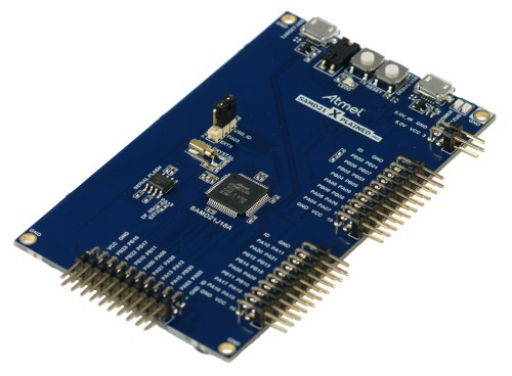
\includegraphics[width=\linewidth]{Figures/sam d21 xplained pro evaluation.png}
        \caption{Carte SAMD21XPLAINEDPRO}
        \label{fig:carte_SAMD21XPLAINEDPRO}
    \end{subfigure}
    \hfill
    \begin{subfigure}[b]{0.48\linewidth}
        \centering
        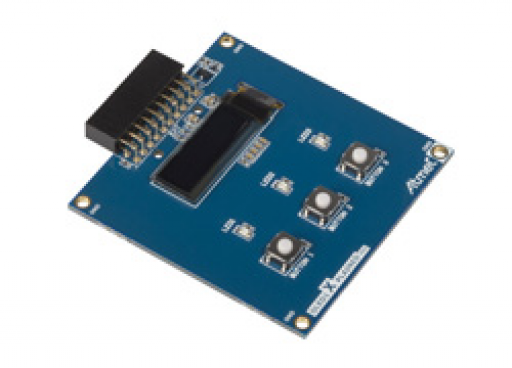
\includegraphics[width=\linewidth]{Figures/oled1 xplained pro extension kit.png}
        \caption{Extension OLED1XPLAINEDPRO}
        \label{fig:extension_OLED1XPLAINEDPRO}
    \end{subfigure}
    \caption{Matériel utilisé pour le système de mesure du temps de réaction}
    \label{fig:materiel_systeme}
\end{figure}

\section{Etude du code FreeRTOS}

\subsection{Clignotement de la LED (Partie 3.4)}

À partir du code fourni en annexe et en suivant les étapes de création du projet sur Microchip Studio, nous avons observé le bon clignotement de la \textit{LED0}. \\

La tâche \textit{Horloge} définit un délai d'attente de 1000 ms (\textit{HORLOGE\_TASK\_DELAY 1000}). L'état de la LED changeant toutes les secondes, un cycle complet (allumé puis éteint) dure 2 secondes. Le système fonctionne donc correctement avec une fréquence de clignotement confirmée de 0,5 Hz.

\begin{lstlisting}[style=code]
void vCodeBlinkLED (void * pvParameters)
{
    /* declaration de variables locales de la tache */
    bool Blink;
    
    /* initialisation des variables locales */
    Blink = false;
    
    for (;;)
    {
        /* attente du semaphore d'eveil */
        xSemaphoreTake (Sem, portMAX_DELAY);
        
        /* Cycle H*/
        if (Blink == false) {
            /* turn LED on. */
            port_pin_set_output_level (LED_0_PIN, LED_0_ACTIVE);
            Blink = true;
        } else {
            /* turn LED off. */
            port_pin_set_output_level (LED_0_PIN, LED_0_ACTIVE);
            Blink = false;
        }
    }
}
\end{lstlisting}

Le résultat de cette exécution sur la carte SAMD21, confirmant la fréquence de clignotement, est visible via ce lien : \href{https://youtu.be/XMjjLOAeuDM}{\textbf{voir la démonstration vidéo sur YouTube}}.

\subsection{Réponses à l'étude du code FreeRTOS (Partie 3.5)}

\begin{itemize}
    \item \textbf{Procédure d'ordonnancement :} Dans le code générique (\textit{tasks.c}), la procédure chargée du changement de contexte et de la sélection de la prochaine tâche à exécuter est \textit{vTaskSwitchContext()} (qui utilise la macro \textit{taskSELECT\_HIGHEST\_PRIORITY\_TASK()}). \\
    
    \item \textbf{Lien avec \textit{FreeRTOSConfig.h} :} La politique d'ordonnancement est directement pilotée par les constantes de ce fichier, principalement \textit{configUSE\_PREEMPTION} (qui active/désactive le mode préemptif) et \textit{configMAX\_PRIORITIES}. \\
    
    \item \textbf{Adaptation de la politique :} Adapter fondamentalement la politique (par exemple vers un ordonnancement de type EDF) n'est pas trivial. Il faudrait directement modifier le code source du noyau dans \textit{tasks.c}, en particulier la procédure \textit{vTaskSwitchContext()} et l'organisation des listes de tâches (\textit{pxReadyTasksLists}). \\
    
    \item \textbf{Politiques de gestion de la mémoire (heap\_1 à heap\_5) :}
    \begin{itemize}
        \item \textit{heap\_1.c} : Allocation uniquement, aucune libération possible (déterministe, idéal pour les systèmes statiques).
        \item \textit{heap\_2.c} : Allocation et libération autorisées, algorithme \textit{best-fit}, mais sans fusion des blocs libres (risque de fragmentation).
        \item \textit{heap\_3.c} : Encapsule les fonctions standards \textit{malloc()} et \textit{free()} du compilateur pour les rendre \textit{thread-safe}.
        \item \textit{heap\_4.c} : Allocation et libération avec fusion automatique des blocs adjacents libres (défragmentation).
        \item \textit{heap\_5.c} : Similaire à \textit{heap\_4.c}, mais permet de répartir le tas (heap) sur plusieurs zones mémoires non contiguës.
    \end{itemize}
\end{itemize}


\section{Contrôle de la fréquence de clignotement de la LED}

Pour modifier la fréquence de clignotement de la LED dans le projet \textit{OLED1}, plusieurs approches sont possibles à partir du code fourni (\textit{mainLeds-BP\_Control.c}) :

\begin{itemize}
    \item \textbf{Modifier la macro de délai (Solution la plus directe) :} La fréquence est régie par la tâche \textit{vCodeClock}, qui s'endort pendant \textit{HORLOGE\_TASK\_DELAY} ticks (défini à 250) avant de libérer le sémaphore \textit{xSem\_H1}. Augmenter ou diminuer la valeur de \textit{HORLOGE\_TASK\_DELAY} modifiera directement la fréquence de basculement de la LED. \\
    
    \item \textbf{Modifier la fréquence du système (Tick Rate) :} La fonction \textit{vTaskDelay()} attend un nombre de "ticks" de l'OS. En modifiant la constante \textit{configTICK\_RATE\_HZ} dans le fichier \textit{FreeRTOSConfig.h} (initialement fixée à 1000 Hz, soit 1 tick = 1 ms), on modifie la durée temporelle réelle d'un tick, et donc la vitesse d'exécution de toutes les tâches temporisées du système. \\
    
    \item \textbf{Ajouter un diviseur logiciel dans la tâche de contrôle :} Dans la tâche \textit{vCodeLEDControl}, au lieu de changer l'état de la LED à chaque réception du sémaphore, on peut introduire un compteur local (variable entière). La LED ne changera d'état que lorsque ce compteur aura atteint un certain seuil, divisant ainsi la fréquence d'horloge.
\end{itemize}

\section{Procédure d'intégration d'un RTOS}

Pour intégrer le code source complet de FreeRTOS dans un projet sous Microchip Studio, il faut suivre les étapes suivantes :

\begin{enumerate}
    \item \textbf{Ajout du noyau générique (Sources et Headers) :} 
    Créer un dossier \verb|FreeRTOS| dans le répertoire \verb|src| du projet et y importer les fichiers sources de base (\verb|tasks.c|, \verb|queue.c|, \verb|list.c|, \verb|timers.c|, \verb|event_groups.c|, \verb|stream_buffer.c|, \verb|croutine.c|). Ces fichiers contiennent la logique du RTOS indépendante du matériel. Créer ensuite un sous-dossier \verb|include| pour y placer tous les fichiers d'en-tête (\verb|.h|) associés. \\

    \item \textbf{Ajout de la couche matérielle (Portage) :} 
    Créer l'arborescence \verb|FreeRTOS/portable/GCC/ARM_CM0| et y importer les fichiers \verb|port.c| et \verb|portmacro.h|. Ces fichiers font le lien direct avec l'architecture du microcontrôleur (Cortex-M0+ de la carte SAMD21) pour gérer les changements de contexte, la pile et les interruptions matérielles. \\

    \item \textbf{Ajout du gestionnaire de mémoire :} 
    Créer le dossier \verb|FreeRTOS/portable/MemMang| et y insérer le fichier définissant la politique d'allocation mémoire dynamique du noyau (ici \verb|heap_1.c|). \\

    \item \textbf{Configuration du noyau (\texttt{FreeRTOSConfig.h}) :} 
    Placer le fichier \verb|FreeRTOSConfig.h| dans le dossier \verb|src/config|. Ce fichier adapte l'OS à l'application en réglant l'horloge CPU (\verb|OSC8M|), la fréquence du tick système (\verb|configTICK_RATE_HZ|), la taille du tas (\verb|configTOTAL_HEAP_SIZE|), le nombre de priorités et la désactivation des fonctions inutilisées (hooks, traces, statistiques). Il fait aussi le lien entre les interruptions du RTOS et celles du processeur (\verb|SysTick_Handler| et \verb|PendSV_Handler|). \\

    \item \textbf{Configuration du compilateur (Include Paths) :} 
    Dans les propriétés du projet (\textit{Toolchain $\rightarrow$ ARM/GNU C Compiler $\rightarrow$ Directories}), ajouter les chemins vers les dossiers \verb|FreeRTOS/include| et \verb|FreeRTOS/portable/GCC/ARM_CM0|. Cela permet au compilateur de trouver tous les fichiers \verb|.h| lors de la compilation.
\end{enumerate}

\section{Application à développer}

\subsection{Contexte}

Cette partie aborde le développement de l'application finale du projet, qui consiste à implanter un système de mesure du temps de réaction. L'objectif est d'évaluer la vitesse de réaction d'un utilisateur à un stimulus visuel géré par la carte SAMD21 et sa carte d'extension OLED1. Le système doit assurer un comportement fonctionnel et temporel rigoureux en s'appuyant sur les mécanismes de l'exécutif FreeRTOS, tels que les tâches, les sémaphores et les files de messages. \\

Le comportement séquentiel et temporel de la fonction centrale d'observation est régi par la machine à états présentée dans la figure ci-dessous. Elle gère les différentes phases du système : le repos, l'attente aléatoire d'un stimulus (allumage de la variable \textit{Sortie} sur les LED), la mesure du temps de réaction de l'utilisateur par comptage d'événements, ainsi que le calcul des statistiques (min, max, moyenne) transmises via une file de messages.

\begin{figure}[h]
    \centering
    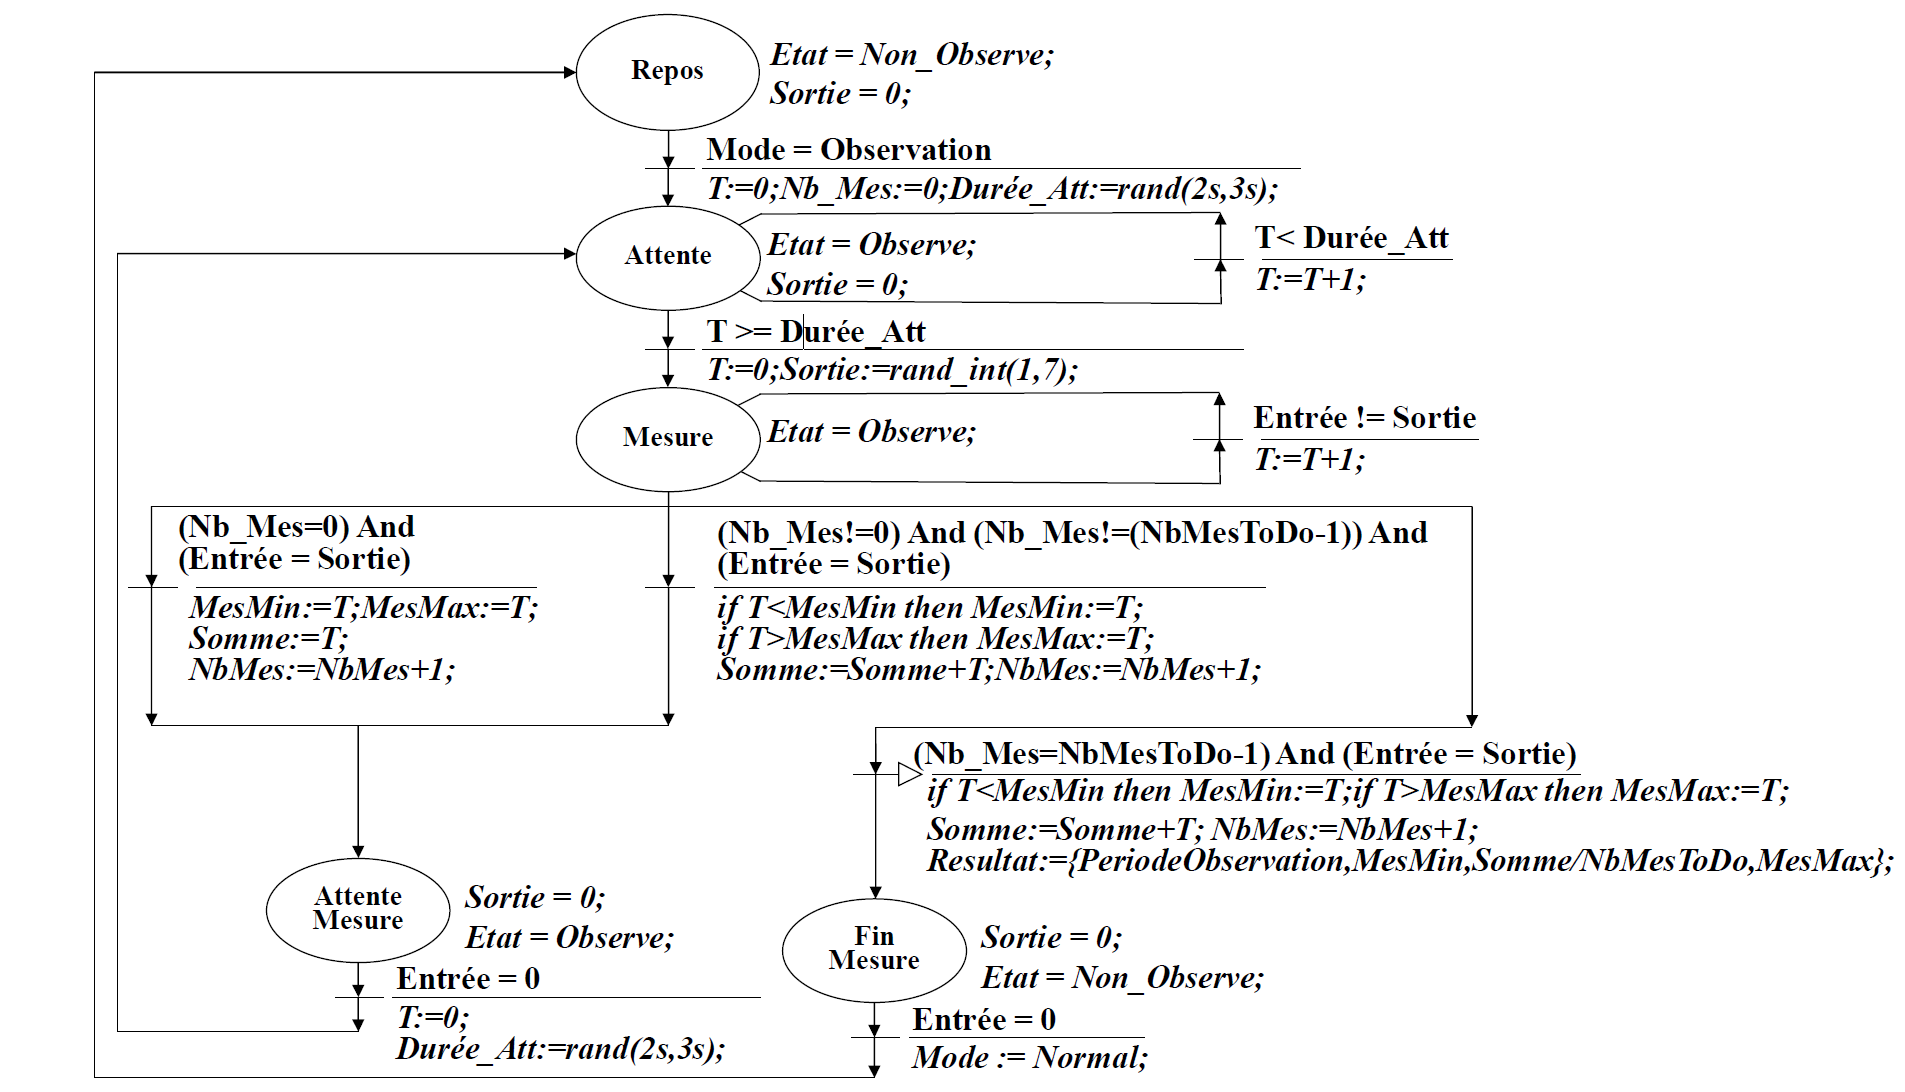
\includegraphics[width=0.8\linewidth]{Figures/fsm_observation.png}
    \caption{Comportement de la fonction Observation (machine à états)}
    \label{fig:machine_etats}
\end{figure}

\subsection{Analyse des besoins en éléments de RTOS pour l'application}

Pour concevoir cette application sous FreeRTOS, l'analyse fonctionnelle met en évidence plusieurs besoins structurants :
\begin{itemize}
    \item \textbf{Tâches (Tasks) :} L'application est découpée en quatre tâches distinctes hiérarchisées par leurs priorités :
    \begin{enumerate}
        \item \texttt{taskClock} (priorité haute) : Tâche périodique (cadencée à $1\text{ ms}$) servant d'horloge globale de référence.
        \item \texttt{taskSupervision} : Tâche chargée de scruter l'état du bouton de démarrage pour basculer en mode observation.
        \item \texttt{taskObservation} : Tâche centrale implémentant l'automate d'état, gérant les stimuli visuels et l'acquisition des boutons.
        \item \texttt{taskDisplay} : Tâche d'affichage passive restituant les statistiques sur l'écran OLED.
    \end{enumerate}
    \item \textbf{Sémaphores binaires :} \texttt{SemSupervision} et \texttt{SemObservation} synchronisent le réveil des tâches sur le tic d'horloge.
    \item \textbf{Mutex (Exclusion Mutuelle) :} \texttt{mutex\_mode} et \texttt{mutex\_oled1} protègent respectivement le mode et les accès concurrents au bus de la carte OLED1.
    \item \textbf{File de messages (Queue) :} \texttt{xQueueMeasurementResults} transfère le tableau des résultats statistiques vers l'affichage.
\end{itemize}

\subsection{Analyse et explication du code de l'application}

Le programme s'articule autour de l'initialisation matérielle (\texttt{system\_init}, \texttt{oled1\_init}, \texttt{ConfigureMeasure}), de la création des objets FreeRTOS, puis du lancement de l'ordonnanceur (\texttt{vTaskStartScheduler}). Le cœur du système repose sur la machine à états de la tâche d'observation (\texttt{REPOS}, \texttt{ATTENTE}, \texttt{MESURE}, \texttt{ATTENTE\_MESURE}, \texttt{FIN\_MESURE}) qui gère l'enchaînement des 5 mesures chronométrées. \\

\subsection{Preuves de fonctionnement de l'application}

Le bon comportement temporel de l'application a été validé sur la cible SAMD21 Xplained Pro avec la carte OLED1, garantissant une période d'observation stable voisine de $1\text{ ms}$. \\

Le résultat de cette exécution sur la carte SAMD21, confirmant le bon fonctionnement de l'application, est visible via ce lien : \href{https://youtube.com/shorts/WNDGfWiWxSI?feature=share}{\textbf{voir la démonstration vidéo sur YouTube}}. \\

\subsection{Code complet de l'application}

Le code source complet de l'application temps-réel FreeRTOS est présenté ci-dessous : \\

\begin{verbatim}
/* Inclusion des bibliothèques */
#include <asf.h>
#include <stdio.h>
#include <string.h>
#include <stdlib.h>
#include "FreeRTOS.h"
#include "task.h"
#include "semphr.h"
#include "timers.h"

#include "oled1.h"
#include "MesTemps.h"
#include "gfx_mono.h"
#include "gfx_mono_text.h"
#include "sysfont.h"

#define OLED1_EXT_HEADER      EXT1
static OLED1_CREATE_INSTANCE(oled1, OLED1_EXT_HEADER);

#define TASK_CLOCK_PRIORITY        (tskIDLE_PRIORITY + 4)
#define TASK_SUPERVISION_PRIORITY  (tskIDLE_PRIORITY + 3)
#define TASK_OBSERVATION_PRIORITY  (tskIDLE_PRIORITY + 2)
#define TASK_DISPLAY_PRIORITY      (tskIDLE_PRIORITY + 1)

#define HORLOGE_TASK_DELAY         1
#define NBMES_TO_DO                5

static SemaphoreHandle_t SemSupervision = NULL;
static SemaphoreHandle_t SemObservation = NULL;
static SemaphoreHandle_t mutex_mode     = NULL;
static SemaphoreHandle_t mutex_oled1    = NULL;
static QueueHandle_t xQueueMeasurementResults = NULL; 

void vSetupHardware(void);
void taskClock(void *pvParameters);
void taskSupervision(void *pvParameters);
void taskObservation(void *pvParameters);
void taskDisplay(void *pvParameters);

typedef enum {
    REPOS,
    ATTENTE,
    MESURE,
    ATTENTE_MESURE,
    FIN_MESURE
} StateForObservation;

typedef enum {
    Normal,
    Observation
} Mode;

static Mode mode = Normal;
static uint16_t measurementResults[4];

static uint16_t T = 0;
static uint16_t Nb_Mes = 0;
static uint16_t Duree_Att = 0;
static uint16_t MesMin = 0;
static uint16_t MesMax = 0;
static uint32_t Somme = 0;
static uint8_t  Sortie_val = 0;

uint8_t get_entree_buttons(void)
{
    uint8_t val = 0;
    if (xSemaphoreTake(mutex_oled1, portMAX_DELAY) == pdTRUE) {
        if (oled1_get_button_state(&oled1, OLED1_BUTTON1_ID)) val |= 0x01;
        if (oled1_get_button_state(&oled1, OLED1_BUTTON2_ID)) val |= 0x02;
        if (oled1_get_button_state(&oled1, OLED1_BUTTON3_ID)) val |= 0x04;
        xSemaphoreGive(mutex_oled1);
    }
    return val;
}

void set_sortie_leds(uint8_t val)
{
    if (xSemaphoreTake(mutex_oled1, portMAX_DELAY) == pdTRUE) {
        oled1_set_led_state(&oled1, OLED1_LED1_ID, (val & 0x01) ? true : false);
        oled1_set_led_state(&oled1, OLED1_LED2_ID, (val & 0x02) ? true : false);
        oled1_set_led_state(&oled1, OLED1_LED3_ID, (val & 0x04) ? true : false);
        xSemaphoreGive(mutex_oled1);
    }
}

void set_etat_led0(bool observe)
{
    if (observe) {
        port_pin_set_output_level(LED_0_PIN, LED_0_ACTIVE);
    } else {
        port_pin_set_output_level(LED_0_PIN, !LED_0_ACTIVE);
    }
}

void vSetupHardware(void)
{
    system_init();       
    gfx_mono_init();     
    oled1_init(&oled1);  
    ConfigureMeasure();  
}

int main(void)
{
    vSetupHardware();

    gfx_mono_draw_filled_rect(0, 0, GFX_MONO_LCD_WIDTH, GFX_MONO_LCD_HEIGHT, GFX_PIXEL_CLR);
    gfx_mono_draw_string("READY - Press SW0", 0, 0, &sysfont);

    srand(1234); 

    SemSupervision = xSemaphoreCreateBinary();
    SemObservation = xSemaphoreCreateBinary();
    mutex_mode     = xSemaphoreCreateMutex();
    mutex_oled1    = xSemaphoreCreateMutex();
    xQueueMeasurementResults = xQueueCreate(1, sizeof(measurementResults));

    xTaskCreate(taskClock,       "Clock",       configMINIMAL_STACK_SIZE,     NULL, TASK_CLOCK_PRIORITY,       NULL);
    xTaskCreate(taskSupervision, "Supervision", configMINIMAL_STACK_SIZE,     NULL, TASK_SUPERVISION_PRIORITY, NULL);
    xTaskCreate(taskObservation, "Observation", configMINIMAL_STACK_SIZE * 2, NULL, TASK_OBSERVATION_PRIORITY, NULL);
    xTaskCreate(taskDisplay,     "Display",     configMINIMAL_STACK_SIZE * 3, NULL, TASK_DISPLAY_PRIORITY,     NULL);

    StartMeasure();
    vTaskStartScheduler();

    for (;;);
}

void taskClock(void *pvParameters)
{
    (void) pvParameters;
    for (;;)
    {
        vTaskDelay(pdMS_TO_TICKS(HORLOGE_TASK_DELAY));
        xSemaphoreGive(SemSupervision);
        xSemaphoreGive(SemObservation);
    }
}

void taskSupervision(void *pvParameters)
{
    (void) pvParameters;
    bool Start;
    bool StartPrec = false;

    for (;;)
    {
        xSemaphoreTake(SemSupervision, portMAX_DELAY);
        Start = (port_pin_get_input_level(BUTTON_0_PIN) == BUTTON_0_ACTIVE);

        if ((StartPrec == false) && (Start == true))
        {
            if (xSemaphoreTake(mutex_mode, portMAX_DELAY) == pdTRUE)
            {
                if (mode == Normal) mode = Observation;
                xSemaphoreGive(mutex_mode);
            }
        }
        StartPrec = Start;
    }
}

void taskObservation(void *pvParameters)
{
    (void) pvParameters;
    StateForObservation PresState = REPOS;
    StateForObservation NextState = REPOS;
    uint16_t periodeObservation_us = 0;

    for (;;)
    {
        xSemaphoreTake(SemObservation, portMAX_DELAY);
        periodeObservation_us = EndMeasure();
        StartMeasure();

        PresState = NextState;

        Mode current_mode = Normal;
        if (xSemaphoreTake(mutex_mode, portMAX_DELAY) == pdTRUE) {
            current_mode = mode;
            xSemaphoreGive(mutex_mode);
        }

        switch (PresState)
        {
            case REPOS:
                set_etat_led0(false);
                set_sortie_leds(0);
                if (current_mode == Observation)
                {
                    T = 0;
                    Nb_Mes = 0;
                    Duree_Att = 2000 + (rand() % 1001);
                    NextState = ATTENTE;
                }
                break;

            case ATTENTE:
                set_etat_led0(true);
                set_sortie_leds(0);
                if (T < Duree_Att)
                {
                    T = T + 1;
                    NextState = ATTENTE;
                }
                else
                {
                    T = 0;
                    Sortie_val = 1 + (rand() % 7);
                    set_sortie_leds(Sortie_val);
                    NextState = MESURE;
                }
                break;

            case MESURE:
            {
                set_etat_led0(true);
                uint8_t entree = get_entree_buttons();

                if (entree != Sortie_val)
                {
                    T = T + 1;
                    NextState = MESURE;
                }
                else
                {
                    if (Nb_Mes == 0)
                    {
                        MesMin = T; MesMax = T; Somme = T;
                        Nb_Mes++; set_sortie_leds(0);
                        NextState = ATTENTE_MESURE;
                    }
                    else if (Nb_Mes < (NBMES_TO_DO - 1))
                    {
                        if (T < MesMin) MesMin = T;
                        if (T > MesMax) MesMax = T;
                        Somme += T; Nb_Mes++; set_sortie_leds(0);
                        NextState = ATTENTE_MESURE;
                    }
                    else
                    {
                        if (T < MesMin) MesMin = T;
                        if (T > MesMax) MesMax = T;
                        Somme += T; Nb_Mes++;

                        measurementResults[0] = periodeObservation_us;
                        measurementResults[1] = MesMin;
                        measurementResults[2] = (uint16_t)(Somme / NBMES_TO_DO);
                        measurementResults[3] = MesMax;

                        xQueueSend(xQueueMeasurementResults, &measurementResults, 0);
                        set_sortie_leds(0);
                        set_etat_led0(false);
                        NextState = FIN_MESURE;
                    }
                }
                break;
            }

            case ATTENTE_MESURE:
                set_sortie_leds(0);
                set_etat_led0(true);
                if (get_entree_buttons() == 0)
                {
                    T = 0;
                    Duree_Att = 2000 + (rand() % 1001);
                    NextState = ATTENTE;
                }
                break;

            case FIN_MESURE:
                set_sortie_leds(0);
                set_etat_led0(false);
                if (get_entree_buttons() == 0)
                {
                    if (xSemaphoreTake(mutex_mode, portMAX_DELAY) == pdTRUE) {
                        mode = Normal;
                        xSemaphoreGive(mutex_mode);
                    }
                    NextState = REPOS;
                }
                break;
        }
    }
}

void taskDisplay(void *pvParameters)
{
    (void) pvParameters;
    char buf[24];
    uint16_t receivedResults[4];

    for (;;)
    {
        if (xQueueReceive(xQueueMeasurementResults, &receivedResults, portMAX_DELAY) == pdTRUE)
        {
            if (xSemaphoreTake(mutex_oled1, portMAX_DELAY) == pdTRUE)
            {
                gfx_mono_draw_filled_rect(0, 0, GFX_MONO_LCD_WIDTH, GFX_MONO_LCD_HEIGHT, GFX_PIXEL_CLR);

                snprintf(buf, sizeof(buf), "Per: %u us", receivedResults[0]);
                gfx_mono_draw_string(buf, 0, 0, &sysfont);

                snprintf(buf, sizeof(buf), "Min: %u ms", receivedResults[1]);
                gfx_mono_draw_string(buf, 0, 8, &sysfont);

                snprintf(buf, sizeof(buf), "Moy: %u ms", receivedResults[2]);
                gfx_mono_draw_string(buf, 0, 16, &sysfont);

                snprintf(buf, sizeof(buf), "Max: %u ms", receivedResults[3]);
                gfx_mono_draw_string(buf, 0, 24, &sysfont);

                xSemaphoreGive(mutex_oled1);
            }
        }
    }
}
\end{verbatim}

\end{document}